\chapter{Background}
Despite the algorithmic simplicity of BFS, achieving high performance execution is a significant challenge on modern multi-core architectures. The primary performance bottleneck is not the algorithm's asymptotical computational complexity, which is linear in the number of vertices and edges, but rather its memory access pattern. The irregular and unpredictable structure of most real-world graphs results in non-contiguous memory accesses, which leads to poor cache utilization and high-latency stalls as the processor waits for data to be fetched from main memory \cite{lenharth2016parallel, lumsdaine2007challenges}. Consequently, state-of-the-art research has largely focused on two areas: refining the traversal strategy itself \cite{arai2024doubling, beamer2013direction, jia2012edge} and redesigning the underlying graph data structures to be more amenable to the memory hierarchies of modern hardware \cite{torok2020improving, iwabuchi2014nvm}.

\section{Direction-Optimizing BFS}
A pivotal advancement in traversal strategy was the introduction of direction-optimizing or Hybrid BFS, proposed by Beamer et al. in 2012 \cite{beamer2013direction}. In a Breadth-First Search, the set of vertices at the current depth of the search is known as the frontier. In this strategy, each frontier expansion is approached either using the Top-Down approach or the Bottom-Up approach. The Top-Down approach, which was used in the other BFS algorithms prior to this work, involves each vertex in the current frontier exploring its neighbors to identify unvisited vertices, which then form the frontier for the next level. The Bottom-Up approach instead inverts the search. It iterates through all vertices and, for those that have not been visited, it checks if they have a parent in the current frontier. A visual representation of both strategies is shown in \cref{fig:hybrid_bfs}. 

\begin{figure}[h]
    \centering
    \includegraphics[width=0.8\linewidth]{images/hybrid bfs.png}
    \caption{Comparison of Top-Down and Bottom-Up Breadth-First Search strategies, starting from source vertex A, for discovering vertices at distance 2. The frontier is the set of vertices at distance 1 $\{B, C, D\}$. The Top-Down approach inspects the neighbors of each vertex in the frontier. This process requires 8 edge traversals to find the next level. However, this strategy performs some superfluous work: it revisits the already visited vertex A, it redundantly traverses the edge C-E even though E was already discovered through B-E, and it unnecessarily traverses edge C-D  and D-C. In contrast, the Bottom-Up approach inspects all unexplored vertices $\{E,F,G\}$, and checks whether any of their neighbors belong to the current frontier $\{B,C,D\}$. This method requires 9 edge traversals, since edges between unexplored vertices (such as E-F, E-G, and F-G) are traversed in both directions.}
    \label{fig:hybrid_bfs}
\end{figure}

\section{Graph diameter and frontier expansions}
The effectiveness of the Top-Down and Bottom-Up strategies is intrinsically linked to a graph's structural properties, most notably its diameter. The diameter dictates the shape and size of the BFS frontier at each level of the traversal, which is the primary factor in determining the most efficient approach \cite{beamer2013direction, andaloro2025cache, arai2024doubling}. This relationship gives rise to two broad classes of graphs: small-diameter and large-diameter.

Small-Diameter Graphs, such as the social networks shown in the plot, are characterized by the "small-world" phenomenon \cite{amaral2000classes}. The frontier size exhibits a distinct pattern: it quickly grows to encompass a significant fraction of the total vertices, and then rapidly collapses. For these graphs, a hybrid traversal is essential. The Top-Down strategy is efficient for the initial and final levels, but during the intermediate phase where the frontier is massive, the Bottom-Up strategy is superior, because it is more efficient to have the small set of unvisited nodes "find" the enormous frontier than the other way around.

Large-Diameter Graphs, such as road networks, Finite Element Models, and Random Geometric Graphs, lack vertices with high degree that create short paths. Consequently, the BFS frontier progresses in a slow, wave-like manner, never "exploding" in size. As shown in the figure, the frontier size for the road networks, FEM and RGG graphs remains relatively small throughout the entire, much longer traversal (the y-axis is logarithmic). For these graphs, the Top-Down approach is almost always the more efficient strategy, as the number of outgoing edges from the frontier is never large enough to justify the high overhead of a Bottom-Up search, which would require iterating over the vast set of unvisited vertices at each step.

This dichotomy in frontier behavior is the core motivation for the direction-optimizing algorithm. The heuristics used to switch between the two modes try to dynamically classify the state of the traversal at each level, applying the Bottom-Up optimization only when the frontier grows large enough to resemble the intermediate state of a small-diameter graph traversal.

\begin{figure}[h]
    \centering
    \includegraphics[width=0.8\linewidth]{images/frontiers_plot.png}
    \caption{The evolution of BFS frontier size for different graphs, colored by their graph class. The plot illustrate the frontier size at each step. Social Networks exhibit an explosive growth and subsequent collapse of the frontier, peaking at over a million vertices in fewer than 100 steps. Road Networks show a very long traversal where the frontier size remains relatively small and stable. Random Geometric Graphs display a steady expansion, confirming its large-diameter nature where the frontier never becomes excessively large. Finite Element Models exhibit intermediate behaviour, they show a more pronounced frontier growth than the road networks, representing a case where a hybrid approach might occasionally activate a Bottom-Up step.}
    \label{fig:frontiersize}
\end{figure}

\section{The Compressed Sparse Row (CSR) format}

The performance of the Top-Down and Bottom-Up traversal strategies is also dependent on the underlying data structure used to represent the graph. A widely adopted and memory-efficient format for representing sparse graphs is the Compressed Sparse Row (CSR) format. The graph's structure is encoded using two primary arrays, called \colidx{} and \rowptr{}. The \colidx{} array contains the concatenated adjacency lists of all vertices. The \rowptr{} array contains the offset of each adjacency list, where the entry at index $i$ points to the start of the $i$-th vertex's adjacency list within the \colidx{} array. The neighbors of a vertex $i$ are therefore located in the segment of the adjacency array delimited by the offsets at index $i$ and $i+1$. An example of the CSR format is shown in the top-right of \cref{fig:csr}. The space complexity of CSR is \bigO{|V| + |E|}, where $|V|$ indicates the number of vertices and $|E|$ indicates the number of edges.

Despite the algorithmic efficiency gained by this hybrid approach, the standard CSR data structure can lead to significant cache inefficiencies. During a traversal, processing a single vertex may require scattered memory accesses to separate arrays: the \rowptr{} for the CSR pointers, the \colidx{} for the neighbor lists, and algorithm-specific data like parent IDs or distances \cite{torok2020improving, andaloro2025cache}. To enhance spatial locality, the MergedCSR format was proposed by Torok \cite{torok2020improving}. This format redesigns the memory layout by merging a vertex's adjacency list into a single, contiguous data structure. By co-locating all data required to process a vertex, this layout minimizes cache misses and reduces pressure on the memory subsystem. An example of the Merged CSR layout is shown in \cref{fig:csr}. The space complexity of MergedCSR is equal to the standard CSR, i.e. \bigO{V + E}. An improvement of the original Merged CSR format is discussed in \cref{sec:mergedcsr}.

\begin{figure}[h]
    \centering
    \includegraphics[width=0.8\linewidth]{images/csr.png}
    \caption{An example of the standard CSR format (top) and a cache-optimized Merged CSR layout (bottom) for the depicted graph. In the Merged CSR format, the hatched cells contain the index of the next vertex's adjacency list. Other cells contain the index of the neighboring vertex inside the Merged CSR. Arrows show the semantics of vertex 1 adjacency list, which has as neighbors vertex 0 (at location 0 in teh MergedCSR array) and vertex 4 (at location 12 in the MergedCSR array). }
    \label{fig:csr}
\end{figure}

While the CSR and MergedCSR formats provide fast retrieval of a vertex's neighbors, which is ideal for the Top-Down step, the Bottom-Up step requires also another lookup: a rapid method to check if a vertex is an element of the frontier.
This check is performed by inspecting the distances array. To facilitate this lookup, some implementations employ a bitmap to store the current frontier to improve cache utilization \cite{beamer2013direction, andaloro2025cache, arai2024doubling, niu2025berrybees}. This is because a bitmap occupies much less space than the distances array: each cell in the distance array requires 32 bits compared to only one bit in the bitmap, increasing the chances of a cache hit.

\section{Parallelization Strategies}
\label{sec:strategies}
To leverage the computational power of multicore processors, the workload of exploring each level of the graph must be distributed across multiple processing cores for concurrent execution. Due to the different structure of the Top-Down and Bottom-Up steps, the two exploration strategies are parallelized differently.

For the Top-Down step, parallelization is achieved by partitioning the current frontier among the available threads. Each thread is assigned a subset of frontier vertices and is responsible for exploring the adjacency lists of its assigned vertices. The primary challenge in this phase is managing concurrent writes to the next frontier.

In the Bottom-Up step, the source of parallelism is the complete set of vertices, which is partitioned among the threads. Each thread iterates through its the vertices in the assigned subset and checks if they are still unvisited by performing a lookup in the bitmap. If so, it checks if any of them is part of the current frontier by performing a lookup in another bitmap.

In both implementations, when multiple threads discover the same unvisited vertex simultaneously, a race condition occurs. To prevent a vertex from being added multiple times, one solution is to use atomic compare-and-swap operations to ensure only one thread successfully marks the vertex and adds it to the frontier \cite{beamer2013direction}. This approach is shown in \cref{fig:paral_shared}. Alternatively, Leiserson and Schardl observed that adding a vertex multiple times to the frontier is a benign race condition that does not affect correctness, but only performance \cite{leiserson2010work}. Their implementation therefore forgoes synchronization, accepting minor redundant work in exchange for lower overhead.

The presence of an inherently sequential data structure such as the next frontier has led to the development of alternative strategies that trade off synchronization overhead with other costs. One common solution to eliminate write contention is having each thread populate its own thread-local frontier queue \cite{beamer2013direction, leiserson2010work}. This avoids the need for atomic operations during the parallel exploration phase but introduces a subsequent merge step at the end of each level, where all thread-local queues must be consolidated into a single frontier for the next iteration. The overhead of this merge phase scales with the number of threads and the number of vertices in the frontier. This approach is shown in \cref{fig:paral_merged}.

A further optimization for the Bottom-Up steps avoids creating an explicit frontier queue by having threads update only the next frontier's bitmap \cite{andaloro2025cache}. The drawback of this `bitmap-only' approach emerges when the algorithm switches from the Top-Down to the Bottom-Up approach or vice versa. This is because the Top-Down step requires an explicit list of frontier vertices to iterate over, necessitating a full scan of the vertex set to reconstruct the frontier from the bitmap. This operation has a cost proportional to the total number of vertices. This approach is shown in \cref{fig:paral_bottomup}.

\begin{figure}[h!]
    \centering

    \begin{subfigure}[c]{0.54\textwidth}
        \centering
        \includegraphics[width=0.8\linewidth]{images/parallelization_shared.png}
        \caption{Shared Frontier with Atomic Operations.}
        \label{fig:paral_shared}
    \end{subfigure}
    
    \vspace{0.5cm}
    
    \begin{subfigure}[c]{0.48\textwidth}
        \centering
        \includegraphics[width=0.8\linewidth]{images/parallelization_merged.png}
        \caption{Thread-Local Frontiers with a Final Merge Step.}
        \label{fig:paral_merged}
    \end{subfigure}
    \begin{subfigure}[c]{0.48\textwidth}
        \centering
        \includegraphics[width=0.9\linewidth]{images/parallelization_bottomup.png}
        \caption{Bitmap-based Approach for Bottom-Up Steps.}
        \label{fig:paral_bottomup}
    \end{subfigure}

    \caption{Proposed approaches for handling parallelization.}
    \label{fig:parallelization}
\end{figure}

\section{Performance Optimizations for Parallel BFS}
\label{sec:optimizations}
This section presents an overview of selected techniques that have been proposed for optimizing the parallel BFS algorithm.

Implementations targeting NUMA systems often employ optimizations which can be relevant also for multicore CPUs. In a NUMA system, each processor (or socket) possesses its own local memory, which offers significantly lower access latency and higher bandwidth compared to accessing memory attached to other processors via high-speed interconnects. Although the algorithms presented in \cref{cha:methodology} focus on multicore CPUs, previous research has shown that also multicore programs benefit from NUMA-like optimizations \cite{blagodurov2010case}. For example, the chiplet architecture of modern AMD EPYC processors and the segmented L3 cache of Intel Cascade Lake results in non-uniform L3 access latency, which varies based on the physical proximity of the accessing core to the cache slice containing the data \cite{velten2022memory}.

The Polymer system \cite{zhang2015numa}, which was one of the first NUMA-aware graph processing systems, co-locates vertices and connected edges within the same NUMA node as much as possible and keeps only a lightweight copy of other vertices' data, such as degree and the start index of neighboring edges. Moreover, they use a Sense-Reversal Centralized Barrier \cite{mellor1991algorithms}, which uses atomic fetch-and-add instructions to reduce contention on the software barrier between each BFS frontier expansion. As for the frontier, they use a variation of thread-local frontiers with a final merge step (as shown in \cref{fig:paral_merged}).

The optimized BFS implementation by Tithi et al. \cite{tithi2013avoiding}, instead focuses on avoiding locks and atomic instructions in shared-memory parallel BFS through optimistic parallelization. This method allows potentially conflicting operations to run in parallel, knowing that conflicts will be rare and manageable without compromising correctness. They implemented the BFS algorithm using both centralized job queues and distributed randomized work-stealing, demonstrating that lock-free versions generally outperform their lock-based counterparts. The authors also discussed strategies for optimizing their algorithms for NUMA machines, such as co-locating threads with their assigned queues on the same socket or prioritizing same-socket work-stealing targets.

Booth and Lane \cite{dennis2022adaptive}, introduced iCh, a loop scheduling method for OpenMP for irregular parallel applications on shared-memory multicore systems. Its key innovations include adaptive self-scheduling using distributed queues per thread and adaptive chunk size tuning that adjusts based on a thread's estimated iteration throughput. It also incorporates an efficient work-stealing mechanism to balance loads. These core ideas, particularly local queues and work-stealing, are directly applicable and beneficial for Breadth-First Search (BFS) implementations, which are also inherently irregular.

The ideas of Sense-Reversal Centralized
Barriers, thread-local queues, and work stealing have been implemented in a single algorithm, described in \cref{sec:pthreads}.

\section{Parallelization Frameworks}

The majority of high-performance BFS implementations for multicore CPUs utilize implicit parallelization through frameworks such as OpenMP \cite{dagum1998openmp} or Cilk++ \cite{leiserson2009cilk++}. Examples include the reference implementation for the Graph500 benchmark up to version 2.1.4 \cite{murphy2010introducing}, the direction-optimizing algorithm by Beamer \cite{beamer2013direction}, the Ligra framework \cite{shun2013ligra}, and the implementations by Tithi et al. \cite{tithi2013avoiding} and Gonzaga et al. \cite{gonzaga2024openmp}. In contrast, more comprehensive graph processing systems such as Polymer \cite{zhang2015numa} and X-Stream \cite{roy2013x} are implemented using the pthreads library\footnote{\url{https://pubs.opengroup.org/onlinepubs/7908799/xsh/pthread.h.html}}, which provides explicit thread management and synchronization. This approach is necessitated by the requirements of these systems, which support numerous graph kernels beyond BFS and often handle dynamic graph updates. Such features demand fine-grained control over memory layout, thread scheduling, and data structure synchronization, a level of control not directly offered by higher-level parallelization frameworks.

Both graph processing systems are more than 10 years old and do not include the direction-optimizing approach. It is therefore of interest to examine the performance of standalone BFS when implemented using explicit parallelization through the pthreads execution model. One such implementation, which includes also the optimizations described in \cref{sec:optimizations}, is discussed in \cref{sec:pthreads}.